%%%%%%%%%%%%%%%%%%%%%%%%%%%%%%%%%%%%%%%%%%%%%%%%%%
%%%%%%%%%%%%%%%%% Documentclass %%%%%%%%%%%%%%%%%%
%%%%%%%%%%%%%%%%%%%%%%%%%%%%%%%%%%%%%%%%%%%%%%%%%%
\documentclass[12pt,				% Font size
			   listof=totoc,		% List of... into table of contents
			   a4paper,				% A4 paper
			   headinclude=false,	% Don't include header into type area calculation
			   footinclude=false,	%
			   headsepline,			% Separating line between header and text
			   DIV=calc,			% Auomatically calculate DIV
			   %BCOR=15mm			% Binding correction
			  ]{scrartcl}

%%%%%%%%%%%%%%%%%%%%%%%%%%%%%%%%%%%%%%%%%%%%%%%%%%
%%%%%%%%%%%%%%%%%%%% Packages %%%%%%%%%%%%%%%%%%%%
%%%%%%%%%%%%%%%%%%%%%%%%%%%%%%%%%%%%%%%%%%%%%%%%%%

% Encoding, fonts, etc...
\usepackage[ngerman]{babel}			% German
\usepackage[utf8]{inputenc}			% Files are UTF-8 encoded
\usepackage[T1]{fontenc}			% Font encoding
\usepackage{lmodern}				% Scalable font
\usepackage{microtype}				% Nicer typesetting
\usepackage{setspace}
%\renewcommand{\ttdefault}{pcr} 	% Monospace font

% Math
\usepackage{amsmath}
\usepackage{amsfonts}
\usepackage{amssymb}
\usepackage{siunitx}				% Allow for german decimals, e.g. 1,344 instead of 1.344 + other stuff

% Graphics, figures, tables...
\usepackage{graphicx}				% Allow graphics
\usepackage{xcolor}					% Allow colors
\usepackage{booktabs}				% Nicer tables
\usepackage{multirow} 				% Make multiple rows one big row in a table
\usepackage{tikz} 					% For generation of vector graphics
\usepackage{pgfplots}				% For nice plots
\usepackage{listings}				% Source code listings
\usepackage{changepage} 			% Margin adjustments for big figures
\usepackage{rotating} 				% Rotate figures if needed
\usepackage{subcaption}				% Figures with multiple images, (a), (b) ...
\usepackage{pdfpages}				% Inserting of full pages from pdf files

% Nice titlepage with more fields for scientific writeups
%\usepackage{titlepage}

% Glossary
%\usepackage{glossaries}			% Can be used to create a nice glossary

% Bibliography, citations...
\usepackage[backend=biber,
			bibstyle=alphabetic,
			citestyle=alphabetic,
			maxbibnames=4,
			firstinits=true,
			hyperref=true,
			backref=true]{biblatex}
\usepackage{url}
\usepackage[babel,
			german=guillemets]{csquotes}
\usepackage{nameref}
\usepackage[plainpages=false]{hyperref}
\usepackage[all]{hypcap}

% other
\usepackage{ifthen}					% Allows conditional statements
\usepackage{blindtext}				% Blindtext for testing purposes

%%%%%%%%%%%%%%%%%%%%%%%%%%%%%%%%%%%%%%%%%%%%%%%%%%
%%%%%%%%%%%%%%%%%%%%% Config %%%%%%%%%%%%%%%%%%%%%
%%%%%%%%%%%%%%%%%%%%%%%%%%%%%%%%%%%%%%%%%%%%%%%%%%

\onehalfspacing

% biblatex
\addbibresource{bibliography.bib}	% Add bibliography file
\DefineBibliographyStrings{ngerman}	% et al. instead of u.a.
	{andothers={et\addabbrvspace al\adddot}}

% titlepage
%\TitlePageStyle[]{KOMAScript}

% TikZ
%\usetikzlibrary{shapes}			% Shapes for Tikz
\usetikzlibrary{plotmarks}			% Plot marks for Tikz
\usetikzlibrary{calc}				% For general calculations
\usetikzlibrary{intersections}		% Can calculate intersections in tikz
\newlength\figureheight 			% Variables for figures exported with matlab2tikz
\newlength\figurewidth
\newcommand\figurescale{1}

% pgfPlots
\pgfplotsset{compat=newest} 
\pgfplotsset{plot coordinates/math parser=false}
\pgfkeys{/pgf/number format/.cd ,use comma ,set thousands separator={ }}

% siunitx
\sisetup{locale = DE}

% listings
\lstset{ %
  backgroundcolor=\color{white},	% background color
  basicstyle=\footnotesize\ttfamily,% code font size
  breakatwhitespace=false,			% automatic breaklines only at whitspaces?
  breaklines=true,					% automatic breaklines
  captionpos=b,						% caption position
  %commentstyle=\color{green},		% comment style
  deletekeywords={},				% delete keywords from language
  escapeinside={(*@}{@*)},          % LaTeX will be evaluated inside (*@ \code{} @*)
  extendedchars=true,				% Non-ASCII characters
  frame=single,						% frame around code
  keepspaces=true,					% keep spaces (i.e. indentation), might need columns = flexible
  %columns=flexible,				% set characters in columns or freely?
  %keywordstyle=\color{blue},       % keyword style
  language=C++,						% programming language
  morekeywords={*,},				% add keywords
  numbers=left,						% line-numbers (none, left, right)
  numbersep=5pt,					% Distance line numbers <-> code
  numberstyle=\tiny\color{gray},	% style for line-numbers
  rulecolor=\color{black},			% frame color
  showspaces=false,					% show spaces by using special underscores?
  showstringspaces=false,			% underline spaces within strings only
  showtabs=false,					% show tabs within strings adding particular underscores
  stepnumber=1,						% step between drawn line-numbers
  %stringstyle=\color{mauve},		% string literal style
  tabsize=4,						% tabs translate to some amount of spaces
  title=\lstname					% Show filename
}
\renewcommand{\lstlistlistingname}{Sourcecodeverzeichnis}

%%%%%%%%%%%%%%%%%%%%%%%%%%%%%%%%%%%%%%%%%%%%%%%%%%
%%%%%%%%%%%%%%%%%% Declarations %%%%%%%%%%%%%%%%%%
%%%%%%%%%%%%%%%%%%%%%%%%%%%%%%%%%%%%%%%%%%%%%%%%%%

% Hyphenation
\hyphenation{Haupt-kom-po-nen-ten-a-na-ly-se Vek-tor-raum Trans-po-nier-ten}

% Math
\newcommand{\var}{\mathrm{Var}}
\newcommand{\cov}{\mathrm{Cov}}
\newcommand{\spur}{\mathrm{Spur}}
\DeclareMathOperator*{\argmin}{arg\,min}
\DeclareMathOperator*{\argmax}{arg\,max}
\DeclareMathSymbol{\mlq}{\mathord}{operators}{``}	% \mlq produces a left quote in math mode
\DeclareMathSymbol{\mrq}{\mathord}{operators}{`'}	% \mrq produces a right quote in math mode

% Text stuff
\newcommand{\highlight}[1]{\emph{#1}}

% Sectioning levels
\newcommand{\sect}[2]{
	\ifthenelse{#1=1}{\chapter{#2}}{
	\ifthenelse{#1=2}{\section{#2}}{
	\ifthenelse{#1=3}{\subsection{#2}}
					 {\subsubsection{#2}}}}
}

% Todo Notes
\newcommand\todo[1]{\textcolor{red}{\textbf{#1}}}
\newcommand\todofoot[1]{\footnote{\textcolor{red}{\textbf{#1}}}}

%%%%%%%%%%%%%%%%%%%%%%%%%%%%%%%%%%%%%%%%%%%%%%%%%%
%%%%%%%%%%%%% Recalculate type area %%%%%%%%%%%%%%
%%%%%%%%%%%%%%%%%%%%%%%%%%%%%%%%%%%%%%%%%%%%%%%%%%
\recalctypearea

\author{Alexander Scheurer}
\title{Portfolio}
\publishers{Hochschule Furtwangen\\Fakultät Digitale Medien}

\begin{document}

\begin{titlepage}
\begin{center}

\Huge
Expos\'{e}\\[-8pt]
\noindent\rule{13.4cm}{0.4pt}\\
\huge
CINEMA 4D als grafischer Editor mit Scriptunterstützung für Fusee\\[-16pt]
\noindent\rule{13.4cm}{0.4pt}\\[24pt]

\normalsize
Alexander Scheurer\\
Baumannstraße 37\\
78120 Furtwangen\\[12pt]
alexander.scheurer@hs-furtwangen.de\\
Matr.-Nr. 248073\\[16pt]

\noindent\rule{9cm}{0.4pt}\\


\large
Hochschule Furtwangen University\\
Fakultät Digitale Medien\\
Studiengang Medieninformatik Master\\[-8pt]
\noindent\rule{9cm}{0.4pt}\\

Forschungsseminar/Wissenschaftliches Arbeiten\\
Prof. Dr. Oliver Ruf\\[-8pt]
\noindent\rule{9cm}{0.4pt}\\
Wintersemester 2014/15\\[60pt]


Version 1\\
Stand: \today

\end{center}
\end{titlepage}

\tableofcontents
\thispagestyle{empty}
\cleardoublepage
%\setcounter{page}{1} 

\section{Abstract}

Bei der Umrechnung von 3D-Objekten in 2D-Bilddaten gehen viele Informationen verloren. Generell ist nur noch die Projektion der Objekte auf die Kameraebene vorhanden, das heißt pixelweise Farbinformationen, also ein Bild. Findet nun eine Interaktion mit diesem Bild statt, z.B. wenn ein Benutzer ein Objekt in der 3D-Szene selektieren möchte, indem er auf dessen Darstellung im Bild klickt, müssen die angeklickten 2D-Kamerakoordinaten auf das dazugehörige Objekt zurück berechnet werden.


Hier gibt es zwei grundverschiedene Ansätze. Einerseits kann hier rein mathematisch aufgelöst werden oder über einen zusätzlichen Renderer, der es mittels Farbiteration möglich macht, eine Relation zwischen Farbe und Objekt herzustellen. Allerdings ist es auch durchaus denkbar, Mischformen dieser Methoden zu entwickeln.


An dieser Stelle setzt die vorliegende Bachelorarbeit an, sie soll die beiden Methoden und mögliche Mischformen vergleichen.


Dazu werden im praktischen Teil der Arbeit, diese Methoden in die Spiele- und Simulations-Engine Fusee\footnote{http://fusee3d.org/} implementiert. Dadurch soll eine objektive Bewertung anhand von numerischen Leistungsvergleichen möglich sein. \cite{Gregory.2010}
\section{Einleitung}

\subsection{Übersicht}

Aktuelle 3D-Grafik-Engines oder auch Spiele-Engines, zum Beispiel \nameref{sec:unity}, Unreal Engine oder CryEngine bieten Spiele-Entwicklern eine grafische Oberfläche (Editor). Im Vergleich zu 3D-Grafiksoftware wie \nameref{sec:c4d} oder 3D Studio MAX, bieten sie allerdings nur sehr beschränkte Möglichkeiten 3D-Objekte zu modellieren/erstellen \cite{Gregory.2014}[S.54]. Das heißt auch, dass je nach dem welche Kombination an 3D-Grafik-Engine und 3D-Grafiksoftware verwendet wird eine Schnittstelle geschaffen werden muss um die Daten (zum Beispiel Geometrie, Texturen, Materialien und Animationen) auszutauschen. \todo{OpenGEX}.

Diese Editoren bieten meist auch eine direkte Schnittstelle zur Programmierung indem Programmcode mit 3D-Objekten verknüpft werden kann.


\subsection{Aufgabe/Fragestellung}

In diesem 
\section{Theoretischer Hintergrund}

\subsection{Fusee}

\begin{figure}[htbp]
  \centering
  \fbox{
    
\includegraphics[width=0.3\textwidth]{images/FuseeLogo375}
  }
  \caption{Fusee Logo}
  \label{fig:FuseeLogo}
\end{figure}

Die Furtwangen University Simulation and Entertainment Engine ist eine 3D-Grafik-Engine, die an der Fakultät Digitale Medien der Hochschule Furtwangen University seit dem Wintersemester 13/14 entwickelt wird. Fusee wird derzeit überwiegend von Studenten im Projektstudium, verschiedenen Wahlpflichtmodulen, Bachelor- sowie Master-Thesen weiter entwickelt. Fusee ist speziell für das Lernen und Lehren im Bereich der 3D-Grafik, Spiele und Simulationen gedacht und ermöglicht in dieser Hinsicht Zugriff auf tiefliegende Funktionen (vergleiche \cite{Muller.2014}).

Grundsätzlich versucht Fusee so viele Plattformen wie möglich zu bedienen. Hierunter zum Beispiel Windows, Linux, Android, iOS und auch HTML5/WebGL fähige Browser. Fusee verfolgt einen hoch modularen Ansatz, jegliche extern anprogrammierte Software und auch teilweise interne bereitgestellte Methoden sollen vom Benutzer der Engine ausgetauscht werden können. Beispiele für Module sind die Grafikanbindung von OpenGL über OpenTK oder die Physikanbindung von Bullet über BulletSharp (siehe \cite{Schey.2014}). Bisher bietet Fusee noch keine Implemtierung von Picking-Verfahren.

\begin{figure}[ht!]
  \centering
  \fbox{
    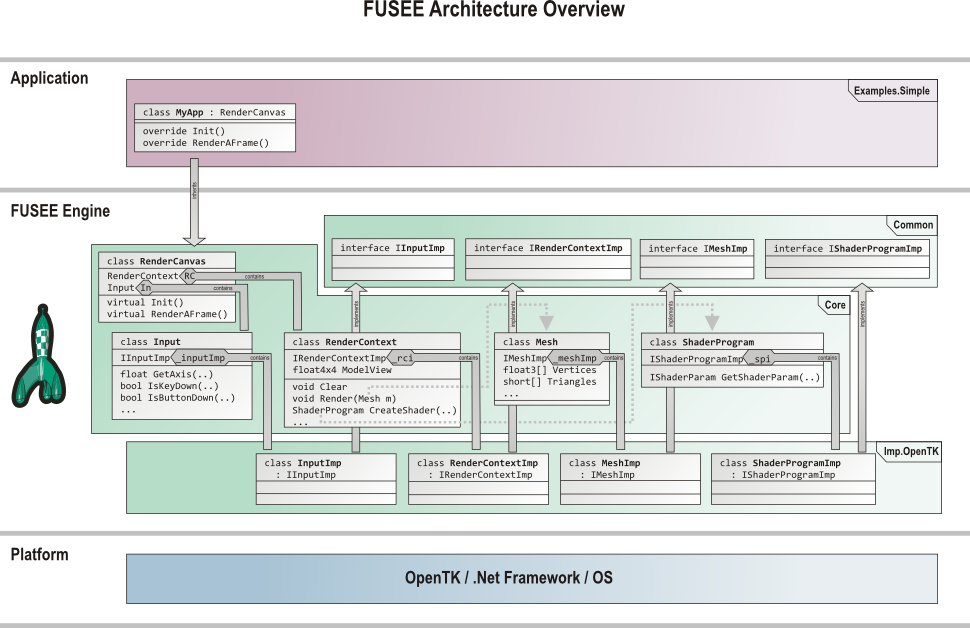
\includegraphics[width=1\textwidth]{images/FuseeArchitecture}
  }
  \caption{Fusee Aufbau}
  \label{fig:FuseeAufbau}
\end{figure}

Seinen modularen Aufbau erreicht Fusee dadurch, dass der Programmcode in drei Bereiche aufgeteilt wird. Der 'Core' beinhaltet alle grundlegenden internen Funktion, der 'Platform Adapter' beinhaltet die Anprogrammierung externen Codes und 'Common' stellt die Funktionalität der Implementierung über Interfaces bereit.

\subsection{Cinema 4D}

\subsection{Unity 3D}
\section{Methodik und Vorgehensweise}

\subsection{Allgemein}
In der Softwaretechnik gibt es etablierte Vorgehensweisen zur Entwicklung von Software. Da hier keine alleinstehende Software entwickelt werden soll, sondern in Abhängigkeit von anderer Software steht, müssen beide Seiten analysiert und passend verbunden werden. Die CINEMA 4D API ist objektorientiert in C++ entwickelt. Fusee hingegen ist zwar auch objektorientiert aufgebaut jedoch in C\# entwickelt. Dadurch liegt nahe, auch das Plugin objektorientiert zu entwickeln. Es muss jedoch die Brücke geschlagen werden zwischen C++ und C\#. Hier muss evaluiert werden in welcher der beiden Sprachen das Plugin entwickelt werden soll und wie es an die jeweils andere Sprache angebunden (gewrappt) werden kann.

Weiterführende Literatur: \cite{Forbrig.2006}, \cite{Buschmann.c2007}, \cite{Gamma.2004}, \cite{Balzert.2001}

\subsection{Werkzeuge}

\subsubsection{Visual Studio}
Visual Studio\footnote{http://www.visualstudio.com/} ist eine Entwicklungsumgebung von Microsoft die mehrere Programmiersprachen, darunter C\# und C++, umfasst. Sowohl Fusee als auch CINEMA 4D werden mit Visual Studio entwickelt.

\subsubsection{ReSharper}
ReSharper\footnote{https://www.jetbrains.com/resharper/} ist eine Erweiterung für Visual Studio von JetBrains. Es erlaubt die Analyse der Programmcode-Qualität und erzwingen eines definierten Programmierstil. Dies macht es einfacher Fehler auch schon während der Entwicklung zu erkennen und durch einen einheitlichen Programmierstil den Programmcode lesbarer und nachvollziehbarer zu machen.

\subsubsection{Git}
Bei der Softwareentwicklung ist von umfangreicheren Projekten eine Versionskontrolle unabdingbar. Sie bietet die Möglichkeit den Entwicklungsvorgang nachzuvollziehen und Fehler bei der Entwicklung, auch weit nach deren Entstehen, zu erkennen. Da das zu erweiternde Fusee Projekt ebenfalls auf Git\footnote{http://git-scm.com/} basiert soll auch in dieser Arbeit geht verwendet werden.
\cite{Loeliger.2012}

\subsubsection{SWIG}
Mit SWIG\footnote{http://www.swig.org/} (Simplified Wrapper and Interface Generator) existiert bereits eine automatisierte Möglichkeit eine Anbindung zwischen C++ und C\# zu ermöglichen. Ohne SWIG würde allein das manuelle Verbinden den Umfang der Arbeit sprengen, es muss lediglich auf beiden Seiten die Voraussetzung für die Anbindung geschaffen werden.
\include{Diskussion}
\section{Wissenschaftliche Einordung}

\subsection{Wissenschaftsgebiet}
Im Hauptteil der Arbeit soll eine Software erweitert werden um die Anbindung an eine zweite Software, dies ist eine überwiegend praktische Ausrichtung und gehört damit ins Feld der praktischen Informatik, genauer der Softwaretechnik.

\subsection{Stand der Forschung}
Im Bereich der Softwaretechnik allgemein ist es nichts Neues, dass Software auch über die Grenzen von Programmiersprachen hinweg miteinander interagiert. Dies kann zum Beispiel Textverarbeitungssoftware sein, die mit einer Spracherkennungssoftware erweitert wird oder Virtualisierungssoftware die es ermöglicht ganze Betriebssysteme miteinander zu verbinden.

In diesem sehr speziellen Bereich der 3D-Computergrafik waren jedoch keine Beispiele zu finden.

\section{Zeitplan}

\begin{itemize}
\item 1 Monat - Literaturrecherche und Auseinandersetzung mit dem Thema
\item 1 Monat - Prototyping der Implementierung
\item 2 Monate - Fertigstellung der Implementierung
\item 1 Monat - Performancetests, Optimierungen und Auswertung
\item 1 Monat - Fertigstellung der Arbeit
\end{itemize}


%LITERATUR

\clearpage
%\appendix

\printbibliography[			% Literaturverzeichnis
	heading=bibintoc,
	title={Literaturverzeichnis}]
%\listoffigures				% Abbildungsverzeichnis
%\listoftables				% Tabellenverzeichnis
%\lstlistoflistings			% Sourcecodeverzeichnis
\end{document}